\documentclass{magnoliaold}

\magtex{tex_driver={pdftex}}
\magfiche{document_nom={Fonctions, flot d'execution},
          auteur_nom={François Fayard},
          auteur_mail={francois.fayard@auxlazaristeslasalle.fr}}
\magexos{exos_matiere={maths},
         exos_niveau={mpsi},
         exos_chapitre_numero={2},
         exos_theme={Flot d'exécution}}
\magmisenpage{misenpage_presentation={tikzvelvia},
         misenpage_format={a4},
         misenpage_nbcolonnes={1},
         misenpage_preuve={non},
         misenpage_sol={non}}
\maglieudiff{}
\magprocess

\begin{document}

%BEGIN_BOOK

\magsection{Programmation procédurale}
\magsubsection{Fonction}

\exercice{nom={Convertir l'heure}}
Écrivez une fonction \verb!conversion_heure(n)! prenant en entrée un entier donnant le
nombre de secondes qui s'est écoulé depuis minuit et renvoyant un \verb!tuple! donnant
l'heure au format heure, minute, seconde. Par exemple \verb!conversion_heure(4567)! devra
renvoyer le tuple \verb_(1, 16, 7)_.

\magsubsection{Liste}
\magsubsection{Ordre d'évaluation}
\magsection{Programmation structurée}
\magsubsection{Branchement}

\exercice{nom={Trier 3 éléments}}
Écrire une fonction \verb!tri(a, b, c)! qui prend en argument trois nombres réels $a$, $b$ et
$c$ et qui renvoie le triplet formé de cet 3 éléments, triés par ordre croissant.

\exercice{nom={Chevauchement}}
Écrire une fonction \verb_chevauche(a, b, c, d)_ prenant en entrée quatre entiers $a$, $b$, $c$ et $d$
et renvoyant \verb_True_ si les segments d'extremités $a$ et $b$ d'une part et $c$ et $d$ d'autre part
ont une intersection non vide.


% \exercice{nom={Moyenne}}
% Écrire un programme initialisant une variable \texttt{note} qui correspond à une moyenne au baccalauréat et renvoyant ensuite la mention s'il y a lieu, le succès ou l'échec à l'examen.

\magsubsection{Boucle for}





% \exercice{nom={Énumérations}}
% \begin{questions}
% \question Écrire une fonction \verb!entiers(i, j)! prenant en entrée deux entiers $i$ et
%   $j$ tels que $i\leq j$ et qui affiche sur une même ligne les entiers de l'intervalle
% 	$\intere{i}{j}$ séparés par le caractère \verb!-!.
% \question Modifier la fonction précédente pour qu'elle affiche désormais les entiers de
%   l'intervalle $\intere{i}{j}$ qui ne sont pas des multiples de 7.
% \end{questions}

\exercice{nom={Graphisme en console}}
\begin{questions}
\question Définir une fonction \verb!triangle1(n)! qui prend en argument un entier $n$
  et qui dessine dans le shell un triangle sur $n$ lignes
\begin{pythoncode}
In [1]: triangle1(5)
(*@\textcolor{purple}{*}@*)
(*@\textcolor{purple}{**}@*)
(*@\textcolor{purple}{***}@*)
(*@\textcolor{purple}{****}@*)
(*@\textcolor{purple}{*****}@*)
\end{pythoncode}
\question Définir une fonction \verb!triangle2(n)! qui dessine ce même triangle mais dans
  l'autre sens.
\begin{pythoncode}
In [2]: triangle2(5)
(*@\textcolor{purple}{*****}@*)
(*@\textcolor{purple}{****}@*)
(*@\textcolor{purple}{***}@*)
(*@\textcolor{purple}{**}@*)
(*@\textcolor{purple}{*}@*)
\end{pythoncode}
\question Définir une fonction \verb!pyramide1(n)! qui dessine une pyramide sur $2n-1$ lignes.
\begin{pythoncode}
In [3]: pyramide1(5)
(*@\textcolor{purple}{*}@*)
(*@\textcolor{purple}{**}@*)
(*@\textcolor{purple}{***}@*)
(*@\textcolor{purple}{****}@*)
(*@\textcolor{purple}{*****}@*)
(*@\textcolor{purple}{****}@*)
(*@\textcolor{purple}{***}@*)
(*@\textcolor{purple}{**}@*)
(*@\textcolor{purple}{*}@*)
\end{pythoncode}
\question Définir une fonction \verb!pyramide2(n)! qui dessine une pyramide de la manière
  suivante.
\begin{pythoncode}
In [4]: pyramide2(5)
    *
   * *
  * * *
 * * * *
* * * * *
\end{pythoncode}
\end{questions}

% \exercice{nom={Le \textsc{Talkhys}}}
% Le \textsc{Talkhys} est un traité d'arithmétique d'\textsc{Ibn Albanna}, mathématicien
% marocain de la première moitié du $13^{\text{e}}$ siècle. On y trouve un certain nombre
% d'identités remarquables.
% \begin{questions}
% \question Écrire un programme reproduisant cette table dans la console.
% \begin{pythoncode}
%         1 x 1         =         1
%        11 x 11        =        121
%       111 x 111       =       12321
%      1111 x 1111      =      1234321
%     11111 x 11111     =     123454321
%    111111 x 111111    =    12345654321
%   1111111 x 1111111   =   1234567654321
%  11111111 x 11111111  =  123456787654321
% 111111111 x 111111111 = 12345678987654321
% \end{pythoncode}
% \question Faire de même avec la table suivante.
% \begin{pythoncode}
% 8 x 1         + 1 = 9
% 8 x 12        + 2 = 98
% 8 x 123       + 3 = 987
% 8 x 1234      + 4 = 9876
% 8 x 12345     + 5 = 98765
% 8 x 123456    + 6 = 987654
% 8 x 1234567   + 7 = 9876543
% 8 x 12345678  + 8 = 98765432
% 8 x 123456789 + 9 = 987654321
% \end{pythoncode}
% \end{questions}

% \exercice{nom={Palindrome}}
% Un palindrome est un mot ou une phrase qui peut se lire indifféremment de la gauche vers
% la droite tels \verb!kayak! ou \verb!eluparcettecrapule!. Écrire une fonction
% \verb!palindrome(s)! qui prend en entrée une chaine de caractères et qui
% renvoie \verb!True! si ce mot est un palindromme et qui renvoie \verb!False! sinon.

\exercice{nom={Le Rot13}}
Le \textsc{Rot13} (rotate by 13 places) est un cas particulier du chiffrage de \textsc{César}.
Comme son nom l'indique, il s'agit d'un décalage de 13 caractères de chaque lettre du texte à
chiffrer~: a devient n, b devient o, c devient p, etc. Son principal aspect pratique est que
le codage et le décodage se réalisent exactement de la même manière puisque notre
alphabet comporte 26 lettres. \textsc{Rot13} est parfois utilisé dans les forums en ligne
comme un moyen de masquer la réponse à une énigme, un spoiler, ou encore une expression
grossière.
\begin{questions}
\question Écrire une fonction \verb!decale(c)! prenant en entrée un caractère et renvoyant
  ce même caractère codé en \textsc{Rot13} si $c$ est un caractère entre \verb!a! et \verb!z!
  et qui renvoie $c$ sinon. On pourra utiliser les fonctions \verb!ord! et \verb!chr!.
\question Définir une fonctin \verb!rot13(s)! prenant en entrée une chaine de caractères et
  renvoyant cette même chaine de caractères codée en \textsc{Rot13}.
\question Utilisez cette fonction pour connaitre la réponse à l'énigme suivante~: Quelle
  est la différence entre un informaticien et une personne normale~?
  \begin{center}
\verb!har crefbaar abeznyr crafr dh'ha xvyb-bpgrg rfg étny à 1000 bpgrgf, ha vasbezngvpvra!
\verb!rfg pbainvaph dh'ha xvybzèger rfg étny à 1024 zègerf!.
  \end{center}
\end{questions}

\exercice{nom={Plus grand plateau}}
On considère une liste \verb!a! dont les éléments sont égaux aux entiers 0 ou 1. Rédiger une fonction
\verb!pg_plateau(a)! calculant le nombre maximal de 0 consécutifs présents dans cette liste. Par exemple,
pour la liste suivante, la fonction devra renvoyer la valeur 7.
\begin{center}
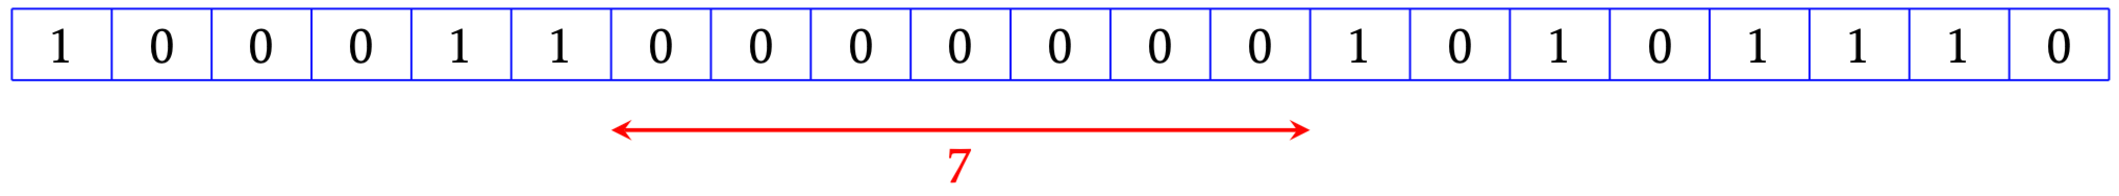
\includegraphics[width=0.8\textwidth]{../../commun/images/python-exo-plateau}\\
\end{center}

\begin{sol}
La fonction suivante répond à la question
\begin{pythoncodeline}
def pg_plateau(a):
    width = 0
    max_width = 0
    for k in range(len(a)):
        if a[k] == 0:
            width = width + 1
            if width > max_width:
                max_width = width
        else:
            width = 0
    return max_width
\end{pythoncodeline}
\end{sol}

\magsubsection{Réduction}

\exercice{nom={Somme}}
Écrire une fonction calculant la somme de tous les entiers inférieurs ou égaux à $n$ inclus
qui sont multiples de $3$ ou de $5$.

\exercice{nom={Suite}}
Écrire une fonction permettant de calculer le $n$-ième terme de la suite définie par
\[\forall n\in\N \qsep u_n\defeq\sum_{k=0}^n \frac{1}{k!}.\]
% On souhaite avoir un affichage de la forme :
% \begin{pythoncode}
% u_10 = ...
% u_11 = ...
% u_12 = ...
% ...
% \end{pythoncode}
% \begin{sol}
% \begin{pythoncode}
% >>> n = 21
%     u = 0
%     for k in range(n):
%         u = u + 1 / math.factorial(k)
%         if k>=10:
%             print("u_" + str(k) + " =", u)
% \end{pythoncode}
% \end{sol}

\exercice{nom={Moyenne, variance}}
 Dans cet exercice, on souhaite calculer la moyenne et la variance d'une liste
  de nombres flottants.
  \begin{questions}
  \question Écrire une fonction \verb!moyenne(t)! qui renvoie la
    moyenne de la liste \verb!t!.
  \question La variance d'une famille finie $t\defeq (t_0,\dots,t_{n-1})$ est donnée par
      \[\mathbb{V}(t)\defeq\frac{1}{n}\sum_{k=0}^{n-1} \p{t_k-\overline{t}}^2\] 
  où $\overline{t}$ est la moyenne de $t$.
  \begin{questions}
  \question Écrire une fonction \verb!variance1(t)! calculant
    la variance de la liste \verb!t!.
  \enonce Cette formule nécessite deux parcours de la liste : un pour calculer $\overline{t}$, et l'autre pour calculer $\mathbb{V}(t)$. Pour calculer $\mathbb{V}(t)$, on peut aussi utiliser la formule de Koenig-Huygens
  \[\mathbb{V}(t)=\cro{\frac{1}{n}\sum_{k=0}^{n-1} t_k^2} -\overline{t}^2.\]
  \question Prouver cette formule.
  \question S'en servir pour écrire une fonction \verb!variance2(t)! qui n'effectue qu'un seul parcours de la liste.
  \end{questions}
  \end{questions}
  \begin{sol}
  \begin{pythoncode}
  def somme(L):
      s=0
      for x in L:
          s=s+x
      return s
  \end{pythoncode}
  \begin{pythoncode}
  def moy(L):
      s=0
      for x in L:
          s=s+x
      return s/len(L)
  \end{pythoncode}
  \begin{pythoncode}
  def var(L):
      n=len(L)
      s,c = 0,0
      for x in L:
          s = s + x
          c = c + x*x
      return c/n - (s/n)*(s/n)
  \end{pythoncode}
  \end{sol}

\exercice{nom={Palindrome}}
Un \emph{palindrome} est un mot pouvant se lire dans les deux sens comme~: radar, rotor, kayak.
Écrire une fonction \verb_palindrome(c)_ qui prend en entrée une chaine de caractères \verb_c_ et qui renvoie le booléen \verb_True_ si cette chaine est un palindrome et \verb_False_ sinon. On rappelle que si \verb_s_ est une chaine de
caractères, on accède au caractère d'indice $k$ grâce à \verb_s[k]_.

\exercice{nom={Monotonie}}
\begin{questions}
\question Écrire une fonction \verb!est_croissante(a)! prenant en entrée une liste d'entiers \verb!a! et renvoyant
  \verb!True! si cette liste est triée dans l'ordre croissant et \verb_False_ sinon.
\question Écrire une fonction \verb!est_monotone(a)! prenant en entrée une liste d'entiers \verb!a! et renvoyant
  \verb!True! si cette liste est triée dans l'ordre croissant ou décroissant et \verb_False_ sinon.
\question Écrivez une fonction répondant à la question précédente mais ne parcourant qu'une seule fois la liste.
\end{questions}



\magsubsection{Boucle while}

% \exercice{nom={Racine carrée entière}}
% La racine carrée entière d'un entier $n\in\N$ est l'unique entier $p$ vérifiant $p^2\leq n<(p+1)^2$.
% \begin{questions}
% \question Rédiger une fonction \verb_isqrt(n)_ qui calcule la racine carrée entière de $n$.
% \question Écrire une deuxième version de cette fonction en ne s'autorisant cette fois que des additions.
% \end{questions}

\exercice{nom={Constante d'Euler}}
On note pour tout $n \in \Ns$
\[S_n\defeq \sum_{k=1}^{n} \frac{1}{k},\qquad
	u_n\defeq S_n-\ln(n) \et v_n\defeq u_n-\frac{1}{n}.\] 
On admet que $(u_n)$ et $(v_n)$ tendent vers la même limite $\gamma$ appelée constante
d'Euler et que l'on a
\[\forall n \in\Ns \qsep v_n \leq \gamma \leq u_n.\]
Écrire une fonction qui calcule un encadrement de $\gamma$ de largeur inférieure à $\epsilon$.
Notre fonction renverra un tuple des deux réels encadrant $\gamma$.



\exercice{nom={Nombre univers}}
On appelle \emph{nombre univers} (en base 10) un nombre réel dont la partie décimale contient
n'importe quelle succession de chiffres de longueur finie. Un exemple simple de nombre
univers en base 10 est la constante de \textsc{Champernowme} $0.123456789101112131415161718192021\ldots$ On pense que $\pi$ est un nombre univers mais
personne n'a pour le moment réussi à le démontrer. De même, on appelle \emph{suite univers} (en base 10) une suite de nombres entiers elle que n'importe quelle succession de chiffres
de longueur finie se trouve dans l'un des termes de cette suite. Il a été prouvé que la
suite des puissances de 2 est une suite univers.
\begin{questions}
\question Écrire une fonction \verb!univers(s)! prenant en entrée une chaine de caractères
  ne comportant que des chiffres et renvoyant la plus petite valeur de $n$ pour laquelle
	\verb!s! est présent dans l'écriture décimale de $2^n$.
\question Déterminer la plus petite puissance de 2 contenant votre date de naissance
  au format \textsc{jjmmaaaa}.
\end{questions}

\exercice{nom={Nombres premiers}}
Le but de cet exercice est de déterminer les 1000 plus petits nombres premiers. Pour
déterminer si un nombre est premier, on utilise le critère suivant~: un entier $p$ est
premier si et seulement si $p\geq 2$ et lorsqu'il n'est divisible par aucun entier
$k$ tel que $2\leq k\leq p$.
\begin{questions}
\question Écrire une fonction \verb!premier(p)! prenant en paramètre un entier $p$ et qui
  renvoie le booléen \verb!True! lorsque $p$ est premier et le booléen \verb!False!
	dans le cas contraire.
\question En remarquant qu'il suffit de montrer que $p$ n'admet aucun diviseur $k$
  tel que $2\leq k$ et $k^2\leq p$ pour montrer que $p$ est premier, écrire une
  nouvelle fonction \verb!premier_bis(p)! plus efficace.
\question Utiliser cette fonction pour afficher les mille plus petits nombres premiers.
\question La conjecture de Goldbach postule que tout entier pair supérieur à 3
  peut s'écrire comme somme de deux nombres premiers (éventuellement égaux). Vérifier
	cette conjecture pour tout entier inférieur où égal à 1000.
\question À contrario, montrer que la conjecture suivante est fausse~: tout nombre impair
  est la somme d'une puissance de 2 et d'un nombre premier.
\end{questions}

\exercice{nom={Suite de Conway}}
Les premiers termes de la suite de Conway sont $1, 11, 21, 1211, 111221,\ldots$
chaque terme étant obtenu en lisant à haute voix le terme précédent. C'est pourquoi
Conway avait baptisé cette suite \emph{look and say}. Par exemple, le terme
1211 se lit \og un 1, un 2, deux 1\fg donc le terme suivant est 111221.
\begin{questions}
\question Écrire une fonction \verb!lookandsay(s)! prenant en paramètre une chaine de
  caractères représentant un entier et renvoyant la chaine de caractère représentant
	l'entier suivant dans la suite de Conway.
\question À l'aide de cette fonction, afficher les 20 premiers termes de la suite de
  Conway.
\question Il a été démontré que si on note $u_n$ le nombre de chiffres du $n$-ième
  nombre de Conway, le rapport $u_{n+1}/u_n$ admet une limite finie $l$.
	Donnez une valeur approchée de $l$.
\question Une autre propriété de cette limite est qu'elle ne dépend pas de la
  valeur initiale (excepté 22). Le vérifier expérimentalement.
\question Démontrer que dans a suite de Conway, ne peuvent apparaitre que les chiffres 1, 2 et 3.
\end{questions}

\magsubsection{Boucles imbriquées}



\exercice{nom={Doublon}}
Écrire une fonction \verb!doublon(a)! prenant en entrée une liste \verb!a! et renvoyant \verb_True_
si \verb_a_ possède un doublon et \verb_False_ sinon. Par exemple, \verb_doublon([3, 4, 7, 3, 2])_
devra renvoyer \verb_True_ car 3 est présent deux fois dans la liste.

\exercice{nom={Somme}}
Écrire une fonction \verb!somme(a, s)! prenant en valeur une liste d'entiers \verb!a! et un entier \verb!s!
et qui renvoie \verb_True_ si $s$ est la somme de deux entiers de la liste $a$ et \verb!False! sinon.
Par exemple \verb!somme([1, 7, 2, 4], 11)! devra répondre \verb!True! car $7+4=11$ et
\verb!somme([1, 7, 2, 4], 14)! devra répondre \verb!False!.

% \exercice{nom={Correction, terminaison}}
% Dans l'exercice qui suit, on pourra pour chacun des programmes écrits justifier sa correction et sa terminaison à l'aide de variants et d'invariants de boucles.
% \begin{questions}
% \question
% Soit la suite $(u_n)$ définie par : $u_0=0$ et, pour tout $n\in\N,u_{n+1}=\sqrt{3+u_n}$.

% \'Ecrire un programme permettant de calculer $u_{100}$.
% \begin{sol}
% \begin{pythoncode}
% import math as m
% u = 0
% for i in range(100):
%     # u contient u_i (vrai pour i = 0)
%     u = m.sqrt(3 + u)
%     # u contient u_{i+1}
% #\`A la fin du dernier tour de boucle, i = 99 donc u contient u_{100}
% print(u)
% \end{pythoncode}
% Boucle for... pas besoin de variants...
% \end{sol}
% \question Soit la suite $(u_n)$ dite de Fibonacci, définie par:
% $\begin{cases}
% u_0=0,u_1=1\\u_{n+2}=u_{n+1}+u_n,\text{ pour }n\in\N
% \end{cases}
% $\\
% \'Ecrire un programme permettant de calculer $u_{100}$.

% \begin{sol}
% \begin{pythoncode}
% u,v=0,1
% for i in range(100):
%     #  u contient u_{i} et v contient u_{i+1} (vrai pour i = 0)
%     u, v = v, u + v
%     #  u contient u_{i+1} et v contient u_{i+2}
% #\`A la fin du dernier tour, i = 99 donc u contient u_{100}
% print(u)
% \end{pythoncode}

% Boucle for... pas besoin de variants...
% \end{sol}
% \question \'Ecrire un programme qui détermine le plus petit entier $n$ tel que $1+2+\dots+n$ dépasse strictement $1000$.
% \begin{sol}
% \begin{pythoncode}
% s = 0
% n = 0
% while s <= 1000:
%     #  s contient 0+...+n (vrai pour n = 0)}
%     n = n + 1
%     #  donc s contient 0+...+(n-1)
%     s = s + n
%     #  s contient 0+...+(n-1)+n
% # ici s > 1000 pour la première fois et s contient $0+\dots+n$
% print(n)
% \end{pythoncode}
% \end{sol}
% \end{questions}


% \exercice{nom={La tortue bourrée}}



% \magsection{Quelques compléments}

% \magsubsection{Fonction}



% \exercice{nom={Paramètres optionnels}}
% Lire l'aide de la fonction \verb_print_ afin de comprendre le rôle des paramètres
% optionnels \verb_sep_ et \verb_end_. En déduire le résultat de l'execution du
% script suivant.
% \begin{pythoncode}
% print(1, 2, 3, sep='+', end='=')
% print(6, 5, 4, sep='\n', end='*')
% \end{pythoncode}

% \magsubsection{Indice, slice}



% \exercice{nom={Mélange de \textsc{Monge}}}
% Le mélange de \textsc{Monge} d'un paquet de cartes numérotées de 1 à $2n$ consiste à
% démarrer un nouveau paquet avec la carte 1, à placer la carte 2 au dessus de ce paquet,
% puis la carte 3 au dessous du nouveau paquet et ainsi de suite en plaçant les cartes
% paires au dessus du nouveau paquet et les cartes impaires au dessous. Autrement dit, si
% le mélange initial est représenté par la suite $(1,2,\ldots,2n)$, son mélange de
% \textsc{Monge} sera représenté par la suite $(2n,2n-2,\ldots,4,2,1,3,5,\ldots,2n-3,2n-1)$.
% Réaliser, à l'aide d'une ligne de \textsc{Python}, le calcul d'un mélange de 
% \textsc{Monge} d'une chaine de caractères \verb_s_.

%END_BOOK

\end{document}
